\documentclass[10.5pt]{article}
\usepackage{longtable}
\usepackage{graphicx}
\usepackage{lineno}
\usepackage{amssymb}
\usepackage{hyperref}
\hypersetup{colorlinks=true, urlcolor=blue, citecolor=black}
\usepackage{natbib}
\usepackage{fullpage}
\usepackage{setspace}
\begin{document}
\begin{flushleft}
{\large
\textbf{Behavioral Genomics: Towards a molecular characterization of individual variation in mammalian social behavior}
}

\vspace{8mm}

\noindent
Matthew D MacManes$^{1,2}$$^\ast$
Anna Geraghty $^{1,4}$
Eileen A Lacey$^{1,3,4}$ \\
\vspace{4mm}


\bf{1} \textnormal{\em{University of California, Berkeley. Berkeley, CA 94720}}  \\
\bf{2} \textnormal{\em{California Institute of Quantitative Biology}} \\
\bf{3} \textnormal{\em{Museum of Vertebrate Zoology}}  \\
\bf{4} \textnormal{\em{Department of Integrative Biology}}  \\

\vspace{4mm}
 
\bf{$\ast$} \textnormal{Corresponding author: \href{mailto:macmanes@gmail.com}{macmanes@gmail.com}, Twitter: \href{https://twitter.com/PeroMHC}{$@$PeroMHC}}
\end{flushleft}

\vspace{8mm}

\begin{abstract}

Elucidating the genetic mechanisms that underlie complex phenotypes is a central problem in modern evolutionary biology. For behavioral biologists, the ability to link allelic differences or variation in gene expression to the occurrence of specific behavioral traits promises to create significant new opportunities to explore the proximate and ultimate bases for variation in animal behavior.  While much progress has been made, mostly in social Hymenoptera, on how allelic differences may lead to interspecific differences in social behavior, whether or not genetics underlie individual variation in behavior is unknown.  Novel high-throughout sequencing techniques provide a newfound ways in which studies of complex traits, particularly in non-model organisms may proceed.  Specifically, the fact that whole transcriptomes can be obtained has allowed us to begin to think about systems and phenotypes where no obvious set of candidate genes exists.  Here, we generate a large Illumina dataset consisting of transcriptomes from 10 social and 10 solitary individuals. Testing for differential expression did not reveal significant differences in expression between the two groups.  While further study is needed, these results provide tantalizing support for the notion that gene expression may not underlie individual differences in behavior, at least in the tuco-tuco, an established model for the study of social behavior. 

\end{abstract}



\doublespacing
\linenumbers

%% main text

\vspace{12mm}

\section*{Introduction}
\hspace{4mm} Elucidating the genetic and genomic mechanisms that underlie complex phenotypes remains a central problem in modern evolutionary biology. In particular, understanding how patterns of allelic variation or gene expression lead to observable differences in phenotypic traits remains a substantial challenge for studies of most organisms. While substantial progress has been made in understanding the genetics of relatively simply phenotypes \citep{Rosenblum:2009ih,Steiner:2007fi}, more complex phenotypes have been challenging (but see \citet{Weber:2009em,Shapiro:2013ce} for examples of research on the genetics of more complex phenotypes). 

For biologists interested complex behavioral phenotypes, the ability to link allelic variation or differences in gene expression to the occurrence of specific behavioral traits promises to create significant new opportunities to explore the proximate and ultimate bases for variation in animal behavior \citep{Blumstein:2010gs}.  Novel high-throughout sequencing techniques provide a newfound ways in which studies of complex traits, particularly in non-model organisms may proceed.  Specifically, the fact that whole transcriptomes can be obtained with relative ease has allowed researchers to begin to think about systems and phenotypes where no obvious set of candidate genes exists.   

Genetic bases for social behavior---Social interactions represent a fundamental component of the behavior of numerous animal species. Accordingly, studies of the adaptive bases for variation in social relationships have long been a focus for behavioral biologists \citep{Alexander:1974va, Allaine:2000uk, Nonacs:2000wa, Fjerdingstad:2006ud, Ebensperger:2008ef}). While research into the genetic underpinnings of social behavior has proceeded more slowly, studies of model laboratory organisms (e.g., \textit{Rattus}, \textit{Mus}) have revealed promising relationships between variation in social relationships and specific genes or gene families \citep{Drew:2007hd, Miyakawa:2003gw, SustkovaFiserova:2009um}. At the same time, studies of less traditional subjects such as prairie voles (\textit{Microtus ochrograster}) are revealing potential links between the formation of pair-bonds and variation at specific loci \citep{Young:1999we, Donaldson:2008cn, Heckel:2008wg}. Pair-bonds may represent a fundamentally different type of social bond (e.g. a sexual relationship) than those characteristic of social systems, and therefore the genetic underpinnings of the social behavior of individuals is virtually unstudied.

In addition to research conducted at the individual level, a substantial amount of work has been done, looking at the genetics of the origins of social behavior \citep{Robinson:2008gq,Toth:2010fr}. This work, focused mostly on the social Hymenoptera, has provided robust support for the idea that genetic changes may somehow participate in the transition from solitary to social life, though the directionality of causation has not been established firmly. Given the fundamental yet complex role that genes play in shaping phenotypic variation, efforts to understand the genetic underpinnings for social interactions are of considerable general interest to behavioral biologists.

Gene expression and behavior. - Studies of gene expression provide a particularly powerful means of linking patterns of behavioral and genetic variation. By comparing rates of gene transcription in individuals that differ with respect to specific phenotypic traits, such studies serve to delineate the genes and gene pathways that underlie the production of particular behavioral phenotypes \citep{Burmeister:2005jw, Mukai:2009cr}. For example such analyses have been used to link aggressive tendencies in mice to differential expression of G-protein coupled neuropeptide receptors such as GABA \citep{SustkovaFiserova:2009um} as well as differential expression of the loci coding for the proteins septin \citep{Suzuki:2009hf} and calcineurin \citep{Miyakawa:2003gw}. Relationships between behavioral variation and patterns of gene expression have also been reported for insects \citep{Toth:2007cr, Dottorini:2007bc} and birds \citep{Mukai:2009cr, Lovell:2008jz, Wacker:2010gg}, thereby underscoring the general importance of such studies for elucidating the genetic underpinnings of social interactions. 

Though studies using a candidate gene approach have been useful in understanding the mechanisms underlying social behavior (e.g. \citep{Fitzpatrick:2005vd}), these studies are fundamentally limited by our current understanding of the genetics of social behavior, which is likely myopic.   Alternatively, the use of a microarray to identify loci that are differentially expressed in individuals displaying distinct behavioral phenotypes may be of value. Indeed, microarrays have been employed to examine behaviorally relevant differences in gene expression in model systems like \textit{Drosophila}, uncovering patterns of expression related to mating behavior in post-copulatory females \citep{Mack:2006cn, McGraw:2004hg} and reproductive success in males \citep{Drnevich:2004dj}.  Like the candidate gene approach, however, constructing microarrays requires a priori knowledge of the sequences of either the specific gene under investigation \citep{Mortazavi:2008jj} or that of a closely related homolog, which limits the suitability of this approach for studies of many non-model organisms. 

Transcriptome sequencing and behavior. - The recent development of high throughput sequencing technologies provides a resolution to the challenges posed by the candidate gene and microarray approaches \citep{Metzker:2010ew, Myles:2010in}.  For studies of complex behavioral traits -- in particular those thought to be mediated by multiple loci or those for which genetic control is completely unknown -- high-throughput sequencing of mRNA represents an emerging opportunity to examine either complete or tissue-specific transcriptomes \citep{VegaArreguin:2009jj, Whittington:2009bn} that can be used to quantify differences in levels of gene expression \citep{Mortazavi:2008jj}. Importantly, this approach does not require \textit{a priori} knowledge of the genes associated with a given behavioral trait, therefore making it particularly promising for studies of non-model organisms. At the same time, the sensitivity of this approach to differences in gene expression suggests that transcriptome sequencing may be used to detect epistatic interactions of the type expected to underlie many complex behavioral phenotypes.  

Given these advantages, we used Illumina sequencing to generate a large mRNA (0.5 billion 100nt and 150nt sequencing reads) dataset from the hippocampi of 20 lab-reared female \textit{Ctenomys sociabilis} that were housed in either social or solitary conditions. Our explicit goals included the identification of genes related to social behavior, and to gain a deeper understanding of the differences in gene expression that may be related to the maintenance of social behavior. 

\section*{Materials and Methods}
\hspace{4mm} Sampling Design. - Whole brains were collected from 20 members of a captive population of colonial tuco-tucos (\textit{Ctenomys sociabilis}) housed on the Berkeley campus. This captive population was founded from 12 free-living individuals captured in Neuquen Province, Argentina, in January, 1996. In captivity, the animals were housed in artificial burrow systems constructed of clear Plexiglas tubes connecting several Plexiglas boxes that served as nest chambers and latrines \citep{Woodruff:2010fc}. Typically, the captive population consisted of approximately 45 individuals. Although the social structure and demographic history of \textit{C. sociabilis} \citep{Chan:2005gj} have resulted in relatively high levels of inbreeding within natural populations of this species, reproductive partners in the captive population were assigned so as to minimize inbreeding within the study subjects.  Animal care and use committee approval was sought and obtained prior to the initiation of this work, and is covered under protocol number R224-2011. 

Twenty unrelated (i.e., non-littermate) females were used in this study. Analyses focused on yearlings as this is the adult age class that is most abundant in nature and that displays the greatest variation in social relationships, ranging from solitary to social lifestyle \citep{Lacey:2004ga}.  Captive females used in this study were housed with 0-3 other adult females, thereby imitating naturally occurring intra-population variation in group size for this species \citep{Lacey:2004ga}. The social groups in which the test animals were housed were stable for at least one month prior to the collection of brain samples.  

Animals were euthanized via overdose with Isoflurane followed immediately by decapitation. The brain was extracted from each individual, after which the hippocampus was dissected out, then placed in a cryotube containing RNAlater (Ambion, Inc), and then flash frozen in liquid nitrogen, and stored at -80C.  RNA was later extracted in a dedicated RNAse-free workspace using a TRIzol extraction (Invitrogen).  mRNA purification and Illumina sequencing library construction was done using the standard TruSeq RNA kit (Illumina) following the manufacturers recommendation.  Each sample was subjected to qPCR using a KAPA kit (Kapa Biosystems, Woburn, MA) for precise quantification. Libraries were then pooled to contain equimolar quantities of each individual library and submitted for Illumina sequencing on a HiSeq 2000 sequencer at The Vincent Coates Genome Sequencing Lab at UC Berkeley.

Assessing sequence quality and pre-assembly procedures. - Accurate assembly of complete transcriptome sequences requires that sequence reads be as error free as possible; random sequencing errors substantially increase the complexity of the \textit{de bruijn} graph, which may result in assembly error \citep{Flicek:2009dl, Miller:2010gx}.   To address this, we used the open-source software package \textsc{Trimmomatic} \citep{Lohse:2012fg} to identify and to trim nucleotides falling below a given quality threshold (PHRED=5) as well as to remove adapter sequences.  To visualize the impact of quality trimming, sequence qualities were assessed pre- and post-quality trimming by the program \textsc{SolexaQA} \citep{Cox:2010ch}. The trimmed quality filtered dataset was then subjected to an error correction pipeline that uses the software package \textsc{Seecer} \citep{Le:2013dy}, recently shown to significantly improve assembly quality \citep{MacManes:2013tv}.  

\textit{De novo} sequence assembly was completed using the program \textsc{Trinity} \citep{Grabherr:2011jb}, which was run on the Pittsburg Supercomputing Center hardware resource Blacklight (\url{http://www.psc.edu/index.php/computing-resources/blacklight}).  This assembly was produced using a solitary individuals (animal ID 406A) whose transcriptome was sequenced with 32M--150nt paired-end Illumina sequencing reads.  These data are available under accession SRR488338 at the Short Read Archive. This assembly strategy was chosen, as opposed to concatenating reads from all individuals, based on recommendations from a recent paper suggesting that approximately 30M reads provides a reasonable balance between depth and sequence error \citep{Francis:2013gc}.

The raw assembly was filtered using multiple methods. First, transcript quantitation was accomplished following a re-mapping strategy implemented in the program eXpress \citep{Roberts:2012dh}. This procedure employs read mapping produced using the ‘very-sensitive-local’ and ‘report all alignments’ settings in Bowtie2 \citep{Langmead:2012jh}.  Low confidence contigs were defined as having FPKM values less than 1 and were removed from the dataset. Second, after deleting low confidence contigs, we attempted to remove contig redundancy. This redundancy can be a product of sequencing error, polymorphism, or alternative splicing; because alternative splicing may have important phenotypic consequences, only very conservative removal of redundant contigs was attempted. To accomplish this, we used the program cd-hit-est \citep{Li:2006hr}, allowing clustering only when 99\% sequence similarity occurred. Finally, we removed sequences corresponding to ribosomal RNA and mitochondrial DNA from the dataset.   

Contig annotation - After \textit{de novo} transcriptome assembly, concatenation, and removal of contaminant and duplicate contigs, we attempted to identify putative transcripts by using a \textsc{BlastN} \citep{Camacho:2009fc} search against the nt database. We then translated putative transcripts from nucleotides to amino acid, and searched for protein coding genes using the \textsc{TransDecoder} software.  We then implemented a \textsc{BlastX} search using the Uniprot database to identify protein coding regions, we well as to determine the completeness of the transcript. Matches were considered significant if the e-value for the sequences compared was \textgreater 10$^{-10}$.  Within the group of significant hits, we chose the best \textsc{Blast} hits based on percent sequence similarity.  We attempted to identify signal peptides that may have secretory function with the software package \textsc{SignalP} \citep{Petersen:2011cn}, and putative transmembrane regions with the program tmhmm \citep{Krogh:2001bv}. Putative transcripts were assigned GO terms using the \textsc{Blast2GO} software package \citep{Conesa:2005hq}. GO terms were then clustered into 3 groups: biological process, molecular function, and cellular component.  

Differential Expression -  Testing for differential expression between the two treatment groups was conducted as follows. Sequencing reads were mapped to contigs contained within the minimally-redundant assembly; the number of reads mapping to each contig was summarized using the program \textsc{eXpress} \cite{Roberts:2012dh}. A data matrix of count data was supplied to the program \textsc{edgeR} \citep{Robinson:2010cw}, in which TMM normalization was completed.  Differential expression was calculated within \textsc{edgeR} after estimating dispersion.  False discovery rate was set at 0.05 using the Benjamini--Hochberg procedure. 

Real-Time Reverse Transcriptase PCR - As a control for assembly and \textit{in silico} transcript abundance estimation, real-time reverse transcriptase PCR was run on TRIzol-extracted RNA further purified with DNase (DNA-free, Ambion). \textit{Rattus} and \textit{Cavia} primers were designed using NCBI Primer BLAST software, which verifies specificity. Tuco-specific primers were designed using partial tuco sequences from Illumina Sequencing results described above. The Ct values were determined using PCR miner \citep{Zhao:2005ku} and normalized to the reference gene, RPLP. For all studies, two-step PCR was used, following the manufacturer’s instructions for iScript cDNA synthesis kit (BioRad) and then the manufacturer’s instructions for SsoAdvanced SYBR supermix (BioRad). Samples were run in a BioRad CFX96 real-time PCR system. After the PCR was complete, specificity of each primer pair was confirmed using melt curve analysis, and all samples run on a 2\% ethidium bromide agarose gel with a 50bp DNA ladder (Invitrogen) to verify correct product size. Primer sequences are available in \hyperlink{Table 1}{Table 1}.

\section*{Results}
\hspace{4mm} In total, 20 individual Illumina sequencing libraries were prepared from the 20 yearling female individuals. Sequencing resulted in over over 500 million 100nt and150nt sequencing reads, distributed over the 20 individuals as per \hyperlink{Table 1}{Table 1}. Sequence read data are available in the SRA. Adapter removal and quality trimming using \textsc{Trimmomatic} resulted in the removal of 3,410,717 reads. \textsc{AllPathsLG} error correction procedures removed an additional 2,491,765 sequence reads, and corrected more that 100 million putative nucleotide errors. Figure 1 illustrate patters of sequence quality prior to \textsc{Trimmomatic} trimming (\hyperlink{Figure 1}{Figure 1A}) as well as post-trimming (\hyperlink{Figure 1}{Figure 1B}), using the sequence reads used for the \textit{de novo} assembly. 

The \textit{de novo} assembly was constructed from 32,541,324--150nt paired-end reads that had been quality trimmed and error corrected. The raw assembly contained 98,239 contigs \textgreater 200nt in length (N50=2,495). Contigs that were not well-supported by sequence reads, as evidenced by having a FPKM \textless 1, were removed from the dataset, as were contigs corresponding to ribosomal RNA and mitochondrial DNA.  After this filtration step, 46,797 contigs remained.  CD-HIT-EST was then used to cluster contigs that were \textgreater 99\% similar, which resulted in the removal of 370 contigs.  After these steps, 46,418 putative transcripts (N50=2,463) remained. The size of the hippocampal transcriptome is estimated to be 53,960,000 nt in size. 

Of the 46,797 contigs, XXX matched a known sequence within the nt database. Approximately 18k putative protein coding regions were discovered, of which YYk were unique. The vast majority of transcripts were full-length, having both start and stop codons \hyperlink{Figure 2}{Figure 2}.  Of these 18k coding regions, 1096 had predicted signal peptides,  and 2877 had putative transmembrane regions.  

Mean and standard deviation of gene expression were calculated for all each gene, using all 20 samples, we well as after partitioning the samples into social and solitary groupings.  The 20 most-highly expressed transcripts, when the mean is calculated using all 20 samples, are listed in \hyperlink{Table 2}{Table 2}. Five of 20 are predicted to contain a transmembrane region, 4 of 20 have a putative signaling peptide region. Nineteen of the 20 most-highly expressed transcripts appear to be coding sequence-- a single sequence comp9226\_c0\_seq1, does not appear to contain an open-reading frame, and may represent a lincRNA or other non-coding transcript.  

            

\section*{Discussion}

\hspace{4mm} Elucidating the genetic and genomic mechanisms that underlie complex phenotypes remains a central problem in modern evolutionary biology. In particular, understanding how patterns of allelic variation or gene expression lead to observable differences in phenotypic traits remains a substantial challenge for studies of most organisms. Although substantial progress has been made in understanding the genetics of the evolution of social behavior \citep{Woodard:2011jv}, understanding how gene underlie individual-level differences in complex phenotypes-- including behavior, remains an outstanding question.  This study attempts to identify the genetic correlates of social behavior in a mammalian system characterized by a flexible social system.  After careful analysis, we were unable to identify significant differences in gene expression. Whether any of the non-significantly different expression profiles are biologically relevant is an unanswered question. \\

\noindent
These results are intriguing-- indeed, ours is one of the 1$^{st}$ to attempt to relate differences in gene expression to differences in complex phenotypes like behavior. Indeed, though we predict that differences exist, it is obviously possible that behavior and other complex phenotypes are fine tuned via a different mechanism.\\

\noindent
In addition to there being a potential biological explanation for our finding, it is possible that we lack statistical power to detect true differences. This seems unlikely, as we were careful to standardize many aspects of animal care, and handled samples in a consistent fashion. We included 10 biological replicates per group, which is well above the typical number of replicates for mRNAseq studies.    \\

\noindent
The brain is not a homogeneous organ-- we now know that discrete regions of the brain are functionally independant. Previous work has suggested that the hippocampus is an important center of behavioral control \citep{Beery:2008do,Pravosudov:2012faa,Weaver:2006by} and therefore we feel confident that had there been changes, this brain area would have been involved.  Future studies looking at different brain regions is in progress. \\

\noindent
Lastly, it could be that mammalian social behavior is hardwired in specific individuals, or is formed in response to stimuli experienced earlier during development. These differences may be observable only during specific developmental stages. We are currently in the process of collecting samples from different developmental stages to gain an ontogenetic perspective on gene expression in the hippocampus.  \\
 



\section*{Acknowledgments}
\noindent


\vspace{10mm}

\singlespacing
\bibliographystyle{model2-names.bst}
\bibliography{formatted.bib}

\section*{Figures \& Tables}

\textbf{\hypertarget{Figure 1}{Figure 1}} \\
\centerline{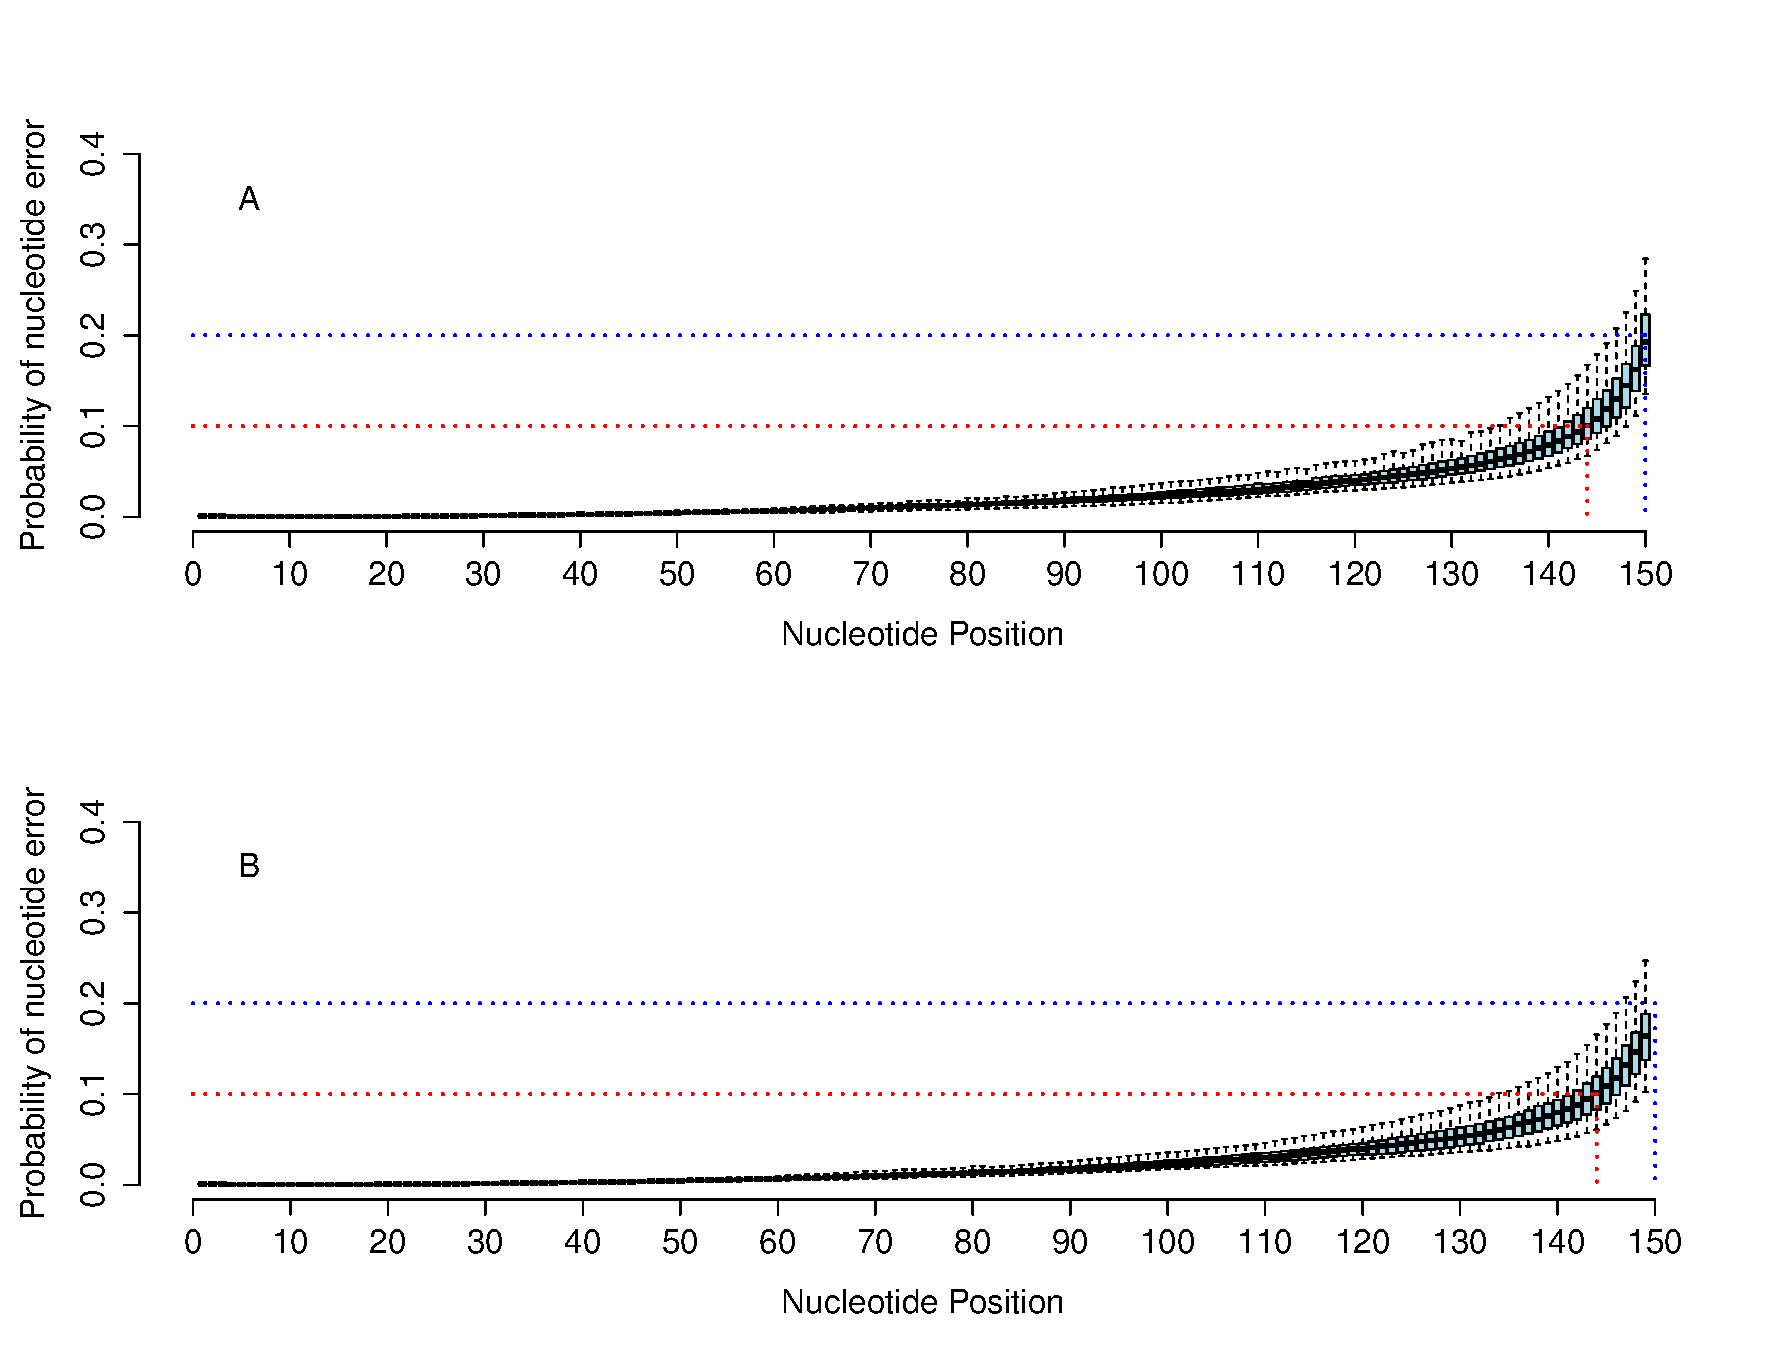
\includegraphics[width=40.0\baselineskip]{Figure1.eps}}


\noindent
Fig. 1. A. The probability of error increases from the 5' to 3' end of the sequencing read. This error pattern is typical of Illumina sequencing.  The red line indicates the 10\% error threshold, which is crossed at the 144$^{th}$ nucleotide. The blue line indicates the 20\% error threshold, which is crossed at the 149$^{th}$ nucleotide. B. Read error profile after trimming. Note that a very gentle trimming has been conducted. 


\vspace{40mm}
\textbf{\hypertarget{Figure 2}{Figure 2}} \\
\centerline{\includegraphics[width=40.0\baselineskip]{Figure2a.eps}}

\noindent
Fig. 2 The vast majority of contigs are full-length transcripts. 

\vspace{40mm}
\textbf{\hypertarget{Figure 3}{Figure 3}} \\
\centerline{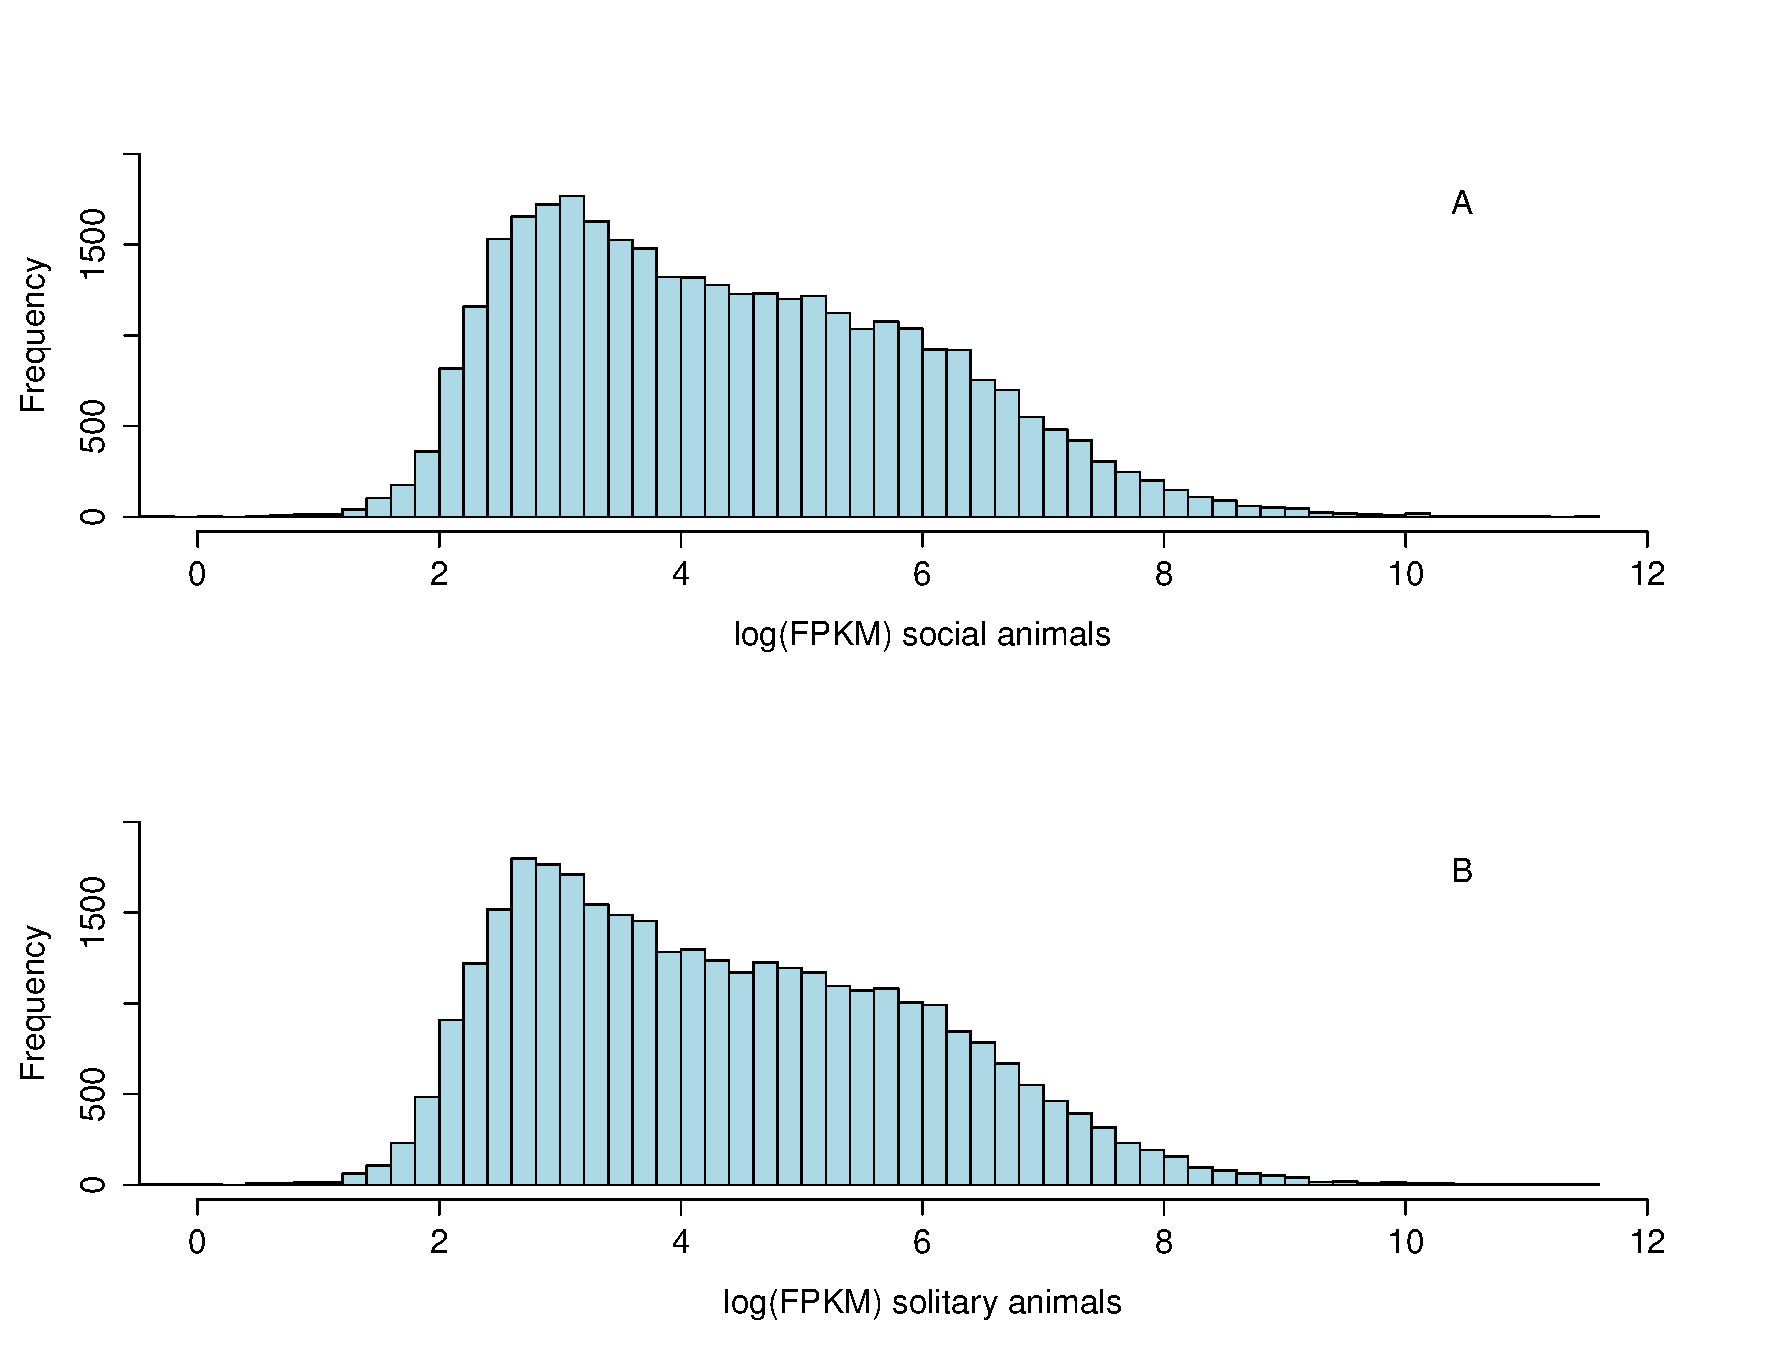
\includegraphics[width=40.0\baselineskip]{Figure3.eps}}

\noindent
Fig. 3 Patterns of expression are similar between social and solitary species. 


\vspace{80mm}

\section*{Table 1}

\textbf{\hypertarget{Table 1}{}} \\
\begin{center}
    \begin{tabular}{ | p{2cm} | p{2cm} | p{3cm}  | p{6cm} |}
    \hline
\textbf{Gene} 	&	 \textbf{Organism} 	&	 \textbf{Forward (F) or Reverse (R)} 	&	 \textbf{Sequence 5' $\rightarrow$ 3'} 	\\ \hline
POMC	&	Rat	&	F	&	CTCACCACGGAAAGCAACCT \\
	&		&	R	&	TTCAGTCAAGGGCTGTTC \\ \hline
CRHBP	&	Rat	&	F	&	GCAGAGGAGCAGCCCTACCG \\
	&		&	R	&	CCCACCCTGGCAGTCCATGG \\ \hline
CRH	&	Rat	&	F	&	GGAGCCGCCCATCTC TCT \\
	&		&	R	&	TCCTGTTGCTGTGAGCTTGCT \\ \hline
CRHR1	&	Rat	&	F	&	TGCAGGCCAGAAACATTGC \\ 
	&		&	R	&	TCCACCTCCCTTCAGGATCA \\ \hline
CRHR2	&	Rat	&	F	&	CTGGAACCTCATCACCACCT \\
	&		&	R	&	AGGTAGCAGCCTTCCACAAA \\ \hline
CRHR2	&	Tuco	&	F	&	CGCCTGGGCCATTGGCAAAC \\ 
	&		&	R	&	TCCACCAGGTCGCCAGGCTC \\ \hline
MR	&	Rat	&	F	&	GTGCGGCTGCAGCTGACCTT \\ 
	&		&	R	&	AGGCCACAGTTCCACGCCAC \\ \hline
GR alpha	&	Rat	&	F	&	ACAGACTTTCGGCTTCTGGA \\ 
	&		&	R	&	CTGAAGATGCATCCGAGTGA \\ \hline
GluR1	&	Rat	&	F	&	CAGATCGATATTGTGAACATCA \\
	&		&	R	&	CCTGAAAGAGCATCTGGTAT \\ \hline
NMDAR1	&	Rat	&	F	&	CTCATCTCTAGCCAGGTCTA \\ 
	&		&	R	&	TCGCATCATCTCAAACCAGAC \\ \hline
RPLP1	&	Rat	&	F	&	ATCTACTCCGCCCTCATCCT \\ 
	&		&	R	&	GCAGATGAGGCTTCCAATGT \\ \hline
 \end{tabular}
\\
\end{center}
\vspace{10mm}
\noindent
Table 1. Primer sequences for quantitative PCR experiments.  

\vspace{10mm}
\section*{Table 2}

\textbf{\hypertarget{Table 2}{}} \\
\begin{center}
    \begin{tabular}{ | p{3.4cm} | p{2.1cm} | p{4cm}  | p{2cm} | p{1.3cm} | p{1.8cm} |}
    \hline
\textbf{Name} 	&	 \textbf{DatabaseID} 	&	 \textbf{Name} 	&	 \textbf{FPKM}  	&	 \textbf{TMM} 	&	\textbf{Signal Peptide}	\\ \hline
comp13664\_c0\_seq1 	&	 P02686 	&	 Myelin basic protein 	&	105199.7	$\pm$	65429	&	0	&	NO	\\ \hline
comp5136\_c1\_seq1 	&	 P02767 	&	 Transthyretin 	&	69252.1	$\pm$	114867	&	0	&	 YES 	\\ \hline
comp5136\_c0\_seq1 	&	 HQ326642 	&	 Calmodulin	&	63590.6	$\pm$	26236	&	0	&	NO	\\ \hline
comp9206\_c0\_seq1 	&	 P26779 	&	 Saposin-A  	&	49256.7	$\pm$	37465	&	0	&	 YES	\\ \hline
comp9199\_c0\_seq1 	&	 P15087 	&	 Carboxypeptidase E	&	48264.4	$\pm$	16964	&	0	&	NO	\\ \hline
comp14077\_c0\_seq1 	&	 Q14515 	&	 SPARC-like protein 1 	&	47868.9	$\pm$	19865	&	0	&	 YES	\\ \hline
comp14063\_c0\_seq1 	&	 P68105 	&	 Elongation factor1-alpha 1	&	45470.5	$\pm$	24411	&	0	&	NO	\\ \hline
comp9202\_c0\_seq1 	&	 Q71U34 	&	 Heat shock cognate 71 kDa protein	&	37875.7	$\pm$	16183	&	0	&	NO	\\ \hline
comp14108\_c0\_seq1 	&	 Q4R4P1 	&	 Heat shock protein HSP 90-alpha	&	37150.7	$\pm$	13513	&	0	&	NO	\\ \hline
comp14104\_c0\_seq1 	&	 Q8TB61 	&	 Adenosine3'-phospho 5'-phosphosulfate transporter 1 	&	33338.4	$\pm$	11724	&	9	&	NO	\\ \hline
comp13104\_c0\_seq1 	&	 P62972 	&	 Polyubiquitin 	&	32834.2	$\pm$	12678	&	1	&	NO	\\ \hline
comp14076\_c0\_seq1 	&	 P04075 	&	 Fructose-bisphosphate aldolase A	&	31671.2	$\pm$	13672	&	0	&	NO	\\ \hline
comp5152\_c0\_seq2 	&	 P60203 	&	 Myelin proteolipid protein 	&	30604.3	$\pm$	16900	&	4	&	NO	\\ \hline
comp11953\_c0\_seq1 	&	 P07214 	&	 SPARC	&	30594.7	$\pm$	15972	&	0	&	NO	\\ \hline
comp9226\_c0\_seq1 	&		&	 ? lincRNA	&	30082.1	$\pm$	9541	&	0	&	NO	\\ \hline
comp14070\_c0\_seq1 	&	 Q4KYY3 	&	 Glyceraldehyde-3-phosphate dehydrogenase	&	29708.9	$\pm$	13529	&	0	&	NO	\\ \hline
comp13888\_c0\_seq1 	&	 P13637 	&	 Sodium/potassium-transporting ATPase subunit alpha-3 	&	25332.9	$\pm$	14498	&	8	&	NO	\\ \hline
comp14068\_c0\_seq1 	&	 P20065 	&	 Thymosin-beta-4	&	25274.4	$\pm$	11164	&	0	&	NO	\\ \hline
comp12851\_c0\_seq3 	&		&	 NDRG4 	&	24781.7	$\pm$	8885	&	0	&	YES	\\ \hline
comp9194\_c0\_seq2 	&	 Q812E9 	&	 Neuronal membrane glycoprotein 	&	24707.6	$\pm$	10530	&	4	&	NO	\\ \hline
 \end{tabular}
\\
\end{center}

\vspace{10mm}
\noindent
Table 2. The twenty most highly expressed genes in the \textit{C. sociabilis} hippocampus. Name refers to the contig ID, while DatabaseID indicates the UniProt transcript identity. FPKM is the estimate of gene expression, averages across the 20 individuals. TMM=transmembrane regions, with the number indicating the of putative transmembrane domains. Signal peptide denotes whether of not a significant signal peptide is discovered, which is often indicative of secretory function.   


\section*{Table 3}
\textbf{\hypertarget{Table 3}{}} \\
\begin{center}
\begin{longtable}{ | l | l | l | l | }
\hline
\textbf{contig name}	&	\textbf{gene name}	&	\textbf{soc (FPKM$\pm$ SD) } & \textbf{sol (FPKM $\pm$ SD)}	 \\ \hline
\endfirsthead
\multicolumn{4}{c}%
{\tablename\ \thetable\ -- \textit{Continued from previous page}} \\
\hline
\textbf{contig name}	&	\textbf{gene name}	&	\textbf{soc (FPKM$\pm$ SD) } &	\textbf{sol (FPKM $\pm$ SD)}			 \\ \hline
\endhead
\hline \multicolumn{4}{r}{\textit{Continued on next page}} \\
\endfoot
\hline
\endlastfoot
comp10487\_c0\_seq1	&	BDNF	&	256	$\pm$	76	&	228	$\pm$	70	 \\ \hline
comp11013\_c0\_seq1	&	Neuroligan-3	&	242	$\pm$	115	&	197	$\pm$	109	\\ \hline
comp12135\_c1\_seq2	&	NEC-1	&	977	$\pm$	409	&	857	$\pm$	368	 \\ \hline
comp12180\_c0\_seq2	&	Neuronal PAS3	&	80	$\pm$	56	&	72	$\pm$	60	 \\ \hline
comp12249\_c0\_seq1	&	NMDA R1	&	1175	$\pm$	809	&	1087	$\pm$	685	\\ \hline
comp12444\_c0\_seq1	&	5-HT2C	&	673	$\pm$	925	&	1312	$\pm$	2144	\\ \hline
comp12616\_c0\_seq2	&	Histone Acetyltransferase p300	&	180	$\pm$	95	&	101	$\pm$	67	 \\ \hline
comp12659\_c0\_seq2	&	PSD-95	&	6851	$\pm$	4701	&	5835	$\pm$	2453	 \\ \hline
comp12745\_c0\_seq2	&	Peroxin-5	&	247	$\pm$	106	&	278	$\pm$	135	 \\ \hline
comp12920\_c1\_seq2	&	Ataxin-3	&	104	$\pm$	44	&	105	$\pm$	46	 \\ \hline
comp13367\_c0\_seq1	&	Guanine Nucleotide Binding Protein	&	99	$\pm$	38	&	95	$\pm$	28	 \\ \hline
comp13702\_c0\_seq12	&	Abelson Interactor 2	&	269	$\pm$	157	&	285	$\pm$	143	\\ \hline
comp14536\_c0\_seq1	&	MAPKK1	&	6096	$\pm$	3119	&	4948	$\pm$	1532	 \\ \hline
comp14614\_c0\_seq1	&	Shank1	&	3387	$\pm$	1423	&	3100	$\pm$	902	 \\ \hline
comp15294\_c0\_seq1	&	MCAD	&	1044	$\pm$	450	&	1324	$\pm$	1068	 \\ \hline
comp16411\_c0\_seq1	&	POMC	&	48	$\pm$	111	&	54	$\pm$	124	 \\ \hline
comp18034\_c0\_seq1	&	PTEN	&	2411	$\pm$	861	&	2454	$\pm$	943	\\ \hline
comp19765\_c0\_seq1	&	ProSAP2	&	239	$\pm$	174	&	226	$\pm$	90	\\ \hline
comp20237\_c0\_seq1	&	CLN8	&	599	$\pm$	331	&	527	$\pm$	218	\\ \hline
comp21149\_c0\_seq1	&	MeCp-2	&	177	$\pm$	66	&	180	$\pm$	73	 \\ \hline
comp21157\_c0\_seq1	&	Caveolin-1	&	195	$\pm$	96	&	202	$\pm$	104	 \\ \hline
comp22526\_c0\_seq1	&	GR	&	483	$\pm$	279	&	535	$\pm$	325	\\ \hline
comp24215\_c0\_seq1	&	Retinoic Acid receptor	&	31	$\pm$	21	&	33	$\pm$	14	 \\ \hline
comp25793\_c0\_seq1	&	CRH-BP	&	136	$\pm$	31	&	139	$\pm$	50	 \\ \hline
comp28662\_c0\_seq1	&	Neuronal Acetylcholine Receptor B2	&	732	$\pm$	419	&	581	$\pm$	215	\\ \hline
comp32945\_c0\_seq1	&	NMDA R2A	&	181	$\pm$	160	&	172	$\pm$	161	 \\ \hline
comp35997\_c0\_seq1	&	Tenascin-R	&	687	$\pm$	539	&	604	$\pm$	494	\\ \hline
comp3934\_c0\_seq2	&	Chorein	&	1217	$\pm$	410	&	1187	$\pm$	417	\\ \hline
comp4697\_c1\_seq1	&	Nuclear Receptor TLX	&	151	$\pm$	44	&	141	$\pm$	32	 \\ \hline
comp49052\_c0\_seq1	&	Dopamine D2 Receptor	&	89	$\pm$	52	&	76	$\pm$	48	 \\ \hline
comp49278\_c0\_seq1	&	NMDA R2B	&	85	$\pm$	46	&	70	$\pm$	46	 \\ \hline
comp51753\_c0\_seq1	&	Caspr4	&	302	$\pm$	113	&	248	$\pm$	100	\\ \hline
comp5378\_c0\_seq1	&	HGPRT	&	149	$\pm$	57	&	160	$\pm$	72	\\ \hline
comp5525\_c0\_seq2	&	Dishevelled-1	&	295	$\pm$	79	&	284	$\pm$	72	 \\ \hline
comp5533\_c0\_seq1	&	JIP-2	&	2631	$\pm$	1359	&	2298	$\pm$	894	 \\ \hline
comp5545\_c0\_seq1	&	Hungtingtin	&	2935	$\pm$	1854	&	2472	$\pm$	1191	 \\ \hline
comp5551\_c0\_seq1	&	nPKC-epsilon	&	7542	$\pm$	3889	&	6562	$\pm$	1839	 \\ \hline
comp6018\_c1\_seq1	&	MR	&	1483	$\pm$	648	&	1429	$\pm$	538	\\ \hline
comp6176\_c0\_seq1	&	Neuroligan-2	&	2668	$\pm$	1527	&	2167	$\pm$	816	 \\ \hline
comp6729\_c0\_seq1	&	Dardarin	&	165	$\pm$	103	&	125	$\pm$	77	\\ \hline
comp7178\_c0\_seq1	&	CRF-R1	&	212	$\pm$	129	&	180	$\pm$	90	\\ \hline
comp72570\_c0\_seq1	&	IL-1	&	49	$\pm$	33	&	48	$\pm$	30	 \\ \hline
comp8432\_c1\_seq2	&	Annexin A3	&	213	$\pm$	163	&	279	$\pm$	267	 \\ \hline
comp9154\_c0\_seq2	&	Junctophillin-3	&	3684	$\pm$	1533	&	3139	$\pm$	849	\\ \hline
comp9338\_c0\_seq1	&	Somatostatin Receptor	&	94	$\pm$	39	&	83	$\pm$	37	 \\ \hline
\end{longtable}
\vspace{5mm}
\end{center}

\vspace{10mm}
\noindent
Table 3. A comparison of the mean gene expression levels ($\pm$ stand. dev.) for solitary and social animals in 45 transcripts previously implicated in social behavior.  \em{Eileen-- I still need to add the qPCR data} 








































\end{document}


